
\subsubsection{Ablaufsteuerung Stateflow (Vorwort für Regelungsstrategie)}
\label{sec:AblaufsteuerungNico}

Um lediglich eine Koordinate anzusteuern und dieses kontinuierlich zu bewegen, wurde eine Koordinate ausgewählt. Über einen Slider kann der Positionswert ausgewählt werden. Die Koordinate wird in das Chart übermittelt. 
Dazu wurde unter anderem die Funktion \textit{buildTargetMsg()} so angepasst, dass nur die Slider-Variable übergeben wird. Die restlichen Koordinaten werden auf die absolute Position der Home-Position gesetzt. Somit bleiben diese beim Starten des Programms auf der Ausgangsposition.
Für die Ansteuerung wurde die Z-Koordinate ausgewählt. Der Vorteil, diese Koordinate anzusteuern, besteht darin, dass man so den Abstand zu der Bodenplatte vorgeben kann. Des Weiteren ist die Anbringung des Sensors für erste Testzwecke einfach \textcolor{red}{(siehe Abbildung~\ref{fig:sensor_anbringung})}. Ebenso werden dabei keine Drehungen des Endeffektors ausgeführt, wie es bei den anderen Koordinaten der Fall gewesen wäre.
Damit der Wert verändert werden kann und man nicht erneut den Start-Button zum Abfahren der Koordinate aktivieren muss, wurde nicht mehr gewartet, bis die Zielposition erreicht wurde, sondern der Write- und Wait-State wurden durch einen einzigen State, den \texttt{MOVE\_STEP}-State, ersetzt. Dieser besitzt eine Junction, die sich selbst wieder aufruft \ref{fig:junction}.

\begin{figure}[h]
    \centering
    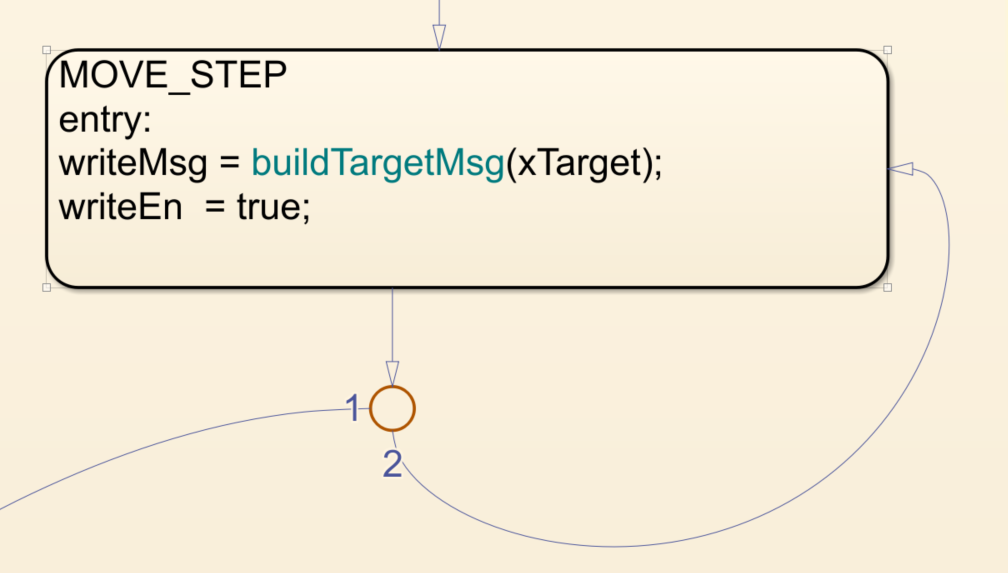
\includegraphics[width=0.3\textwidth]{images/junction.png}
    \caption{Selbstwiederaufruf des MOVE\_STEP-States mit priorisierter Stopp-Bedingung bei Unterschreitung eines Schwellwertes.}
    \label{fig:junction}
\end{figure}


Um rechtzeitig reagieren zu können, falls die ausgewählte Position zu groß ist und der Roboter in eine gefährliche Position fährt, wird die Position schrittweise übergeben. Damit ist es möglich, den Not-Stopp rechtzeitig zu drücken.
\\
Die Schrittweite wurde durch einen Saturation-Block begrenzt. In diesem kann man einstellen, wie groß der maximale Wert sein darf, der weitergeleitet wird. Alle Werte darunter werden unverändert weitergeleitet.
Da dadurch nur noch relative Schritte gemacht werden, wurde die Strecke zu einer integrierenden Strecke erweitert. Die Schritte, die aus dem Saturation-Block kommen, werden auf die aktuelle Position des Roboters aufaddiert.

\subsection{Zusammenführung von Sensorik und Roboterkommunikation}

Durch den \textit{HIL-Read}-Block wurde der Sensor in das Steuerungsprogramm implementiert. Da die DSP(Digital Signal Processing)-Toolbox für den Medianfilter nicht zur Verfügung stand, wurde dieser in einem \textit{MATLAB Function}-Block nachgebildet. Somit konnten die kalibrierten Sensorwerte in das Programm eingebracht werden.

Durch das schrittweise Anfahren an die Sollposition ist es möglich, einen Mindestabstand zu implementieren. Wird dieser unterschritten, wird der \texttt{MOVE\_STEP}-State verlassen und vor der nächsten Bewegung muss erneut der Start-Button aktiviert werden. Damit diese Funktion Priorität besitzt, ist die entsprechende Bedingung als erste Junction eingetragen (vgl. Abbildung~\ref{fig:junction}).

Zunächst wurden die Sensorausgabewerte simuliert. Dies ist ebenfalls mittels eines Sliders geschehen, sodass auch hier die Sensorwerte manuell dynamisch geändert werden konnten. Damit konnte sich der Ausgabewert langsam an den Sollwert anpassen, wodurch das Heranfahren simuliert wurde.


\subsubsection{Entwicklung der Regelungsstrategie}
Der Sollabstand, den der Endeffektor einhalten soll, wird über eine Konstante vorgegeben, die über einen Slider einstellbar ist. 

Für die Regelung wird die Differenz zwischen Sollabstand und Sensorwert auf die Ist-Koordinate aufaddiert. Somit wird die absolute Position als Ziel-Position des MOVE\_STEP-States übergeben. Da direkt die absoluten Positionen übermittelt werden, wird die Differenz ohne zusätzliche Verstärkung weitergeleitet \textcolor{red}{überprüfen ob das so stimmt-Laborversuch (P1 oder P 0.05)}.

Auf diese Weise wird die Differenz direkt auf die Koordinate berechnet und der Endeffektor wird in der Simulation ohne Überschwingen an die Position geführt. Durch die integrierende Strecke tritt kein Positionsfehler auf, weshalb kein zusätzlicher I-Regler benötigt wird. \textcolor{red}{bzw mit leichtem Überschwingen - Laborversuch}. 


Im realen Versuch war die Armbewegung stotternd, was auf die Kombination aus dem \textit{Saturation}-Block und der Befehlsübertragung zurückzuführen ist, da so der Arm auf den nächsten Befehl wartet. 

Da der reale Sensor trotz des Medianfilters Schwankungen von $\pm\qty{2}{\cm}$ aufwies, zeigte der Endeffektor trotz Erreichen der Soll-Position leichte Ausgleichsbewegungen.
Aufgrund dessen wurde dem Regler ein \textit{Dead-Zone}-Block vorgeschaltet. Damit hält der Endeffektor seinen Abstand innerhalb eines bewusst akzeptierten Toleranzbands von 2 cm ein, ohne auf Sensorrauschen mit Ausgleichsbewegungen zu reagieren. Dies stellt einen gezielten Kompromiss zwischen Positionsgenauigkeit und Regelstabilität dar.

Des Weiteren neigte das System zu einem leichten Überschwingen \textcolor{red}{(siehe Abbildung~\ref{fig:ueberschwingen_realer_sensor} falls nicht reproduzierbar weglassen?)}.

\bigskip
Um eine flüssigere Bewegung zu erreichen, wurde der \textit{Saturation}-Block entfernt. Es wurde vermutet, dass der Arm dadurch direkt und stotterfrei auf die Sollposition fährt. Jedoch kam es dabei zu einem starken Überschwingen und einer langen Einpendeldauer \textcolor{red}{(siehe Abbildung~\ref{fig:signale}) - Laborversuch wiederholen wenn realer Sensor funktioniert}.



 \begin{figure}[h]
    \centering
    \begin{subfigure}[b]{0.48\textwidth}
        \centering
        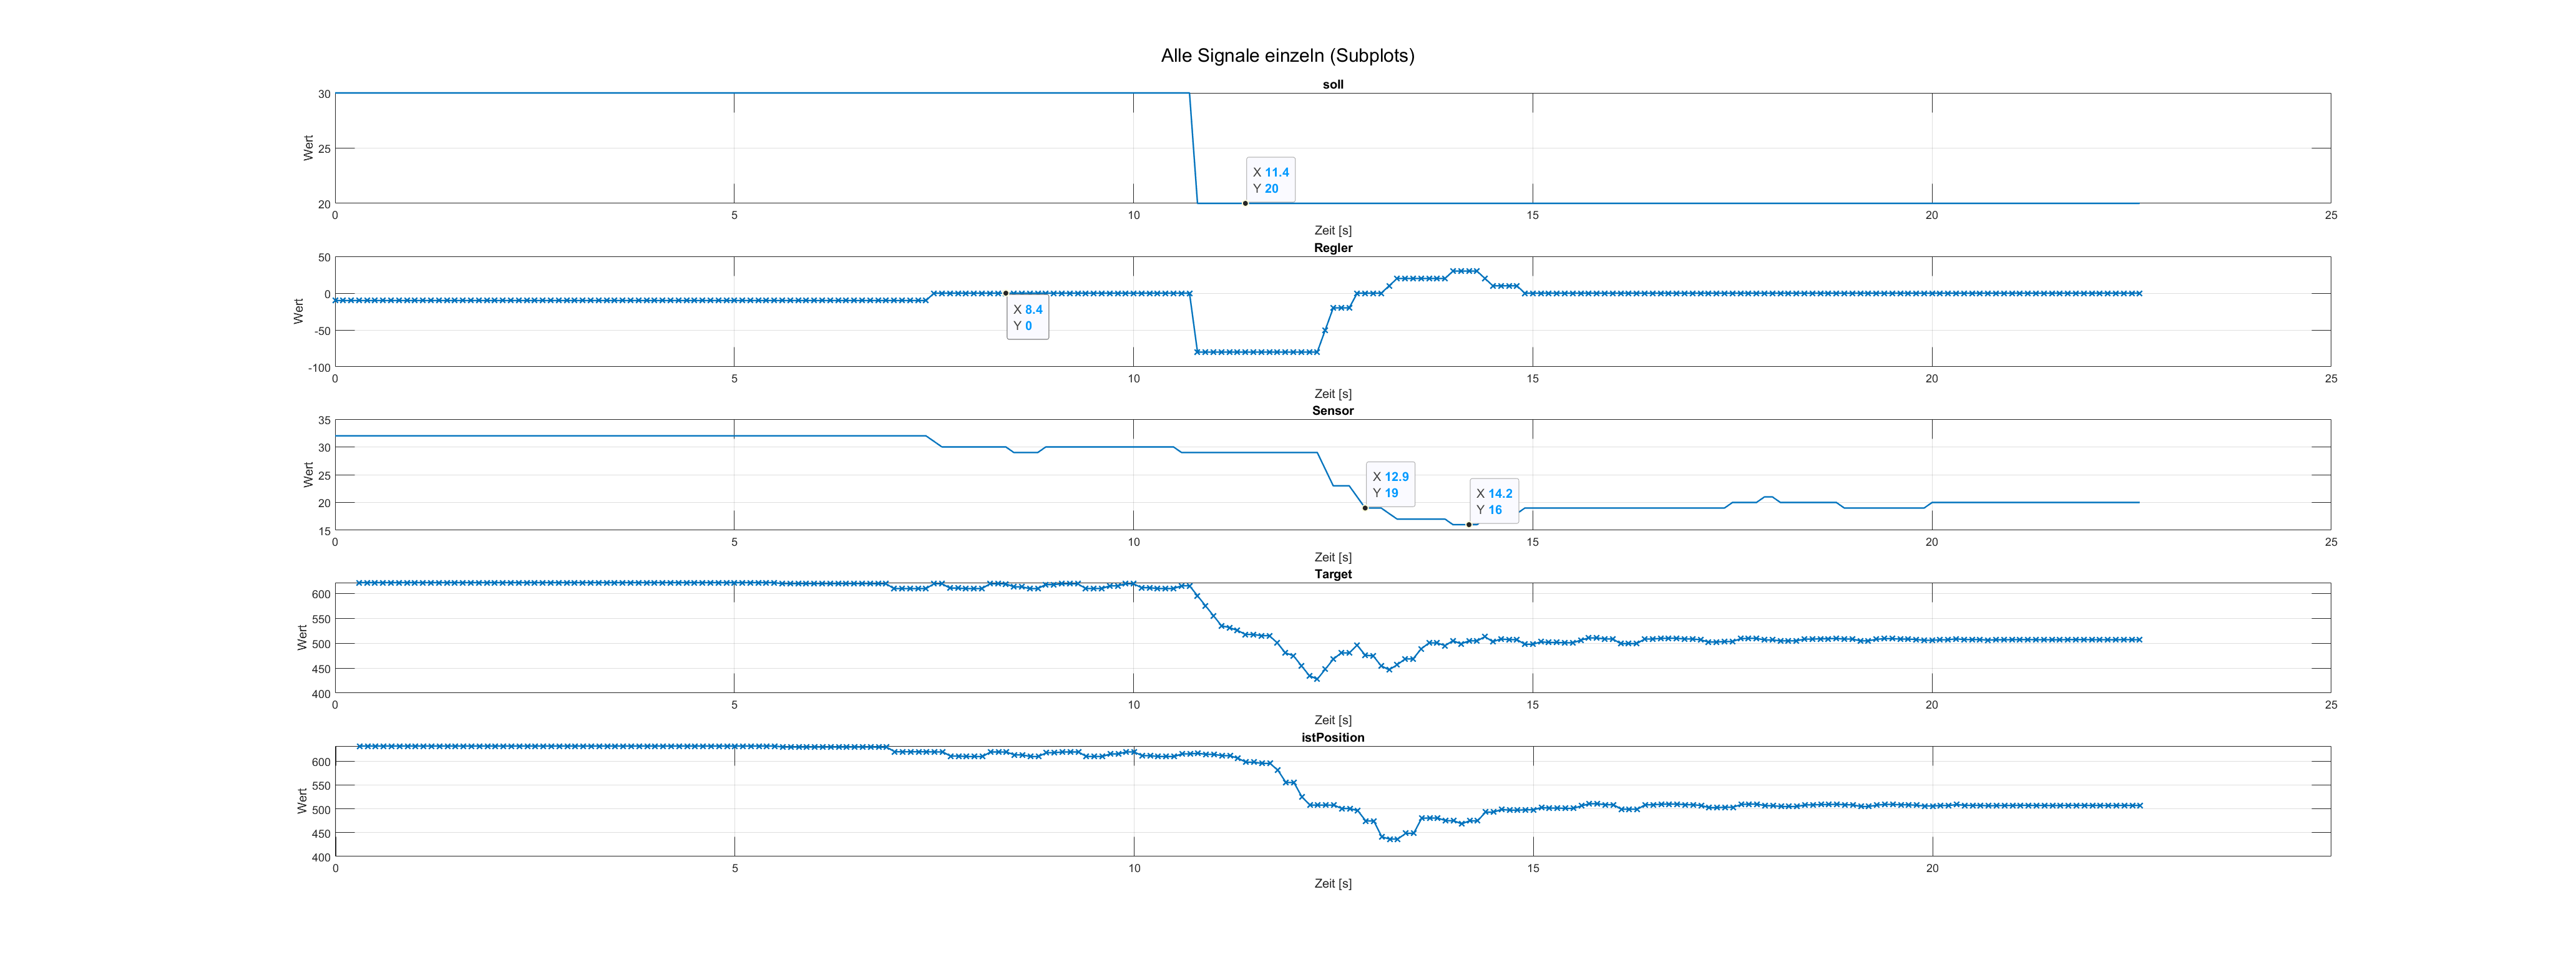
\includegraphics[width=\textwidth]{images/signaleEInzeln.png}
        \caption{Bild der einzelnen Signale}
        \label{fig:signaleEinzeln} % Label für Teilbild (a)
    \end{subfigure}
    \hfill
    \begin{subfigure}[b]{0.48\textwidth}
        \centering
        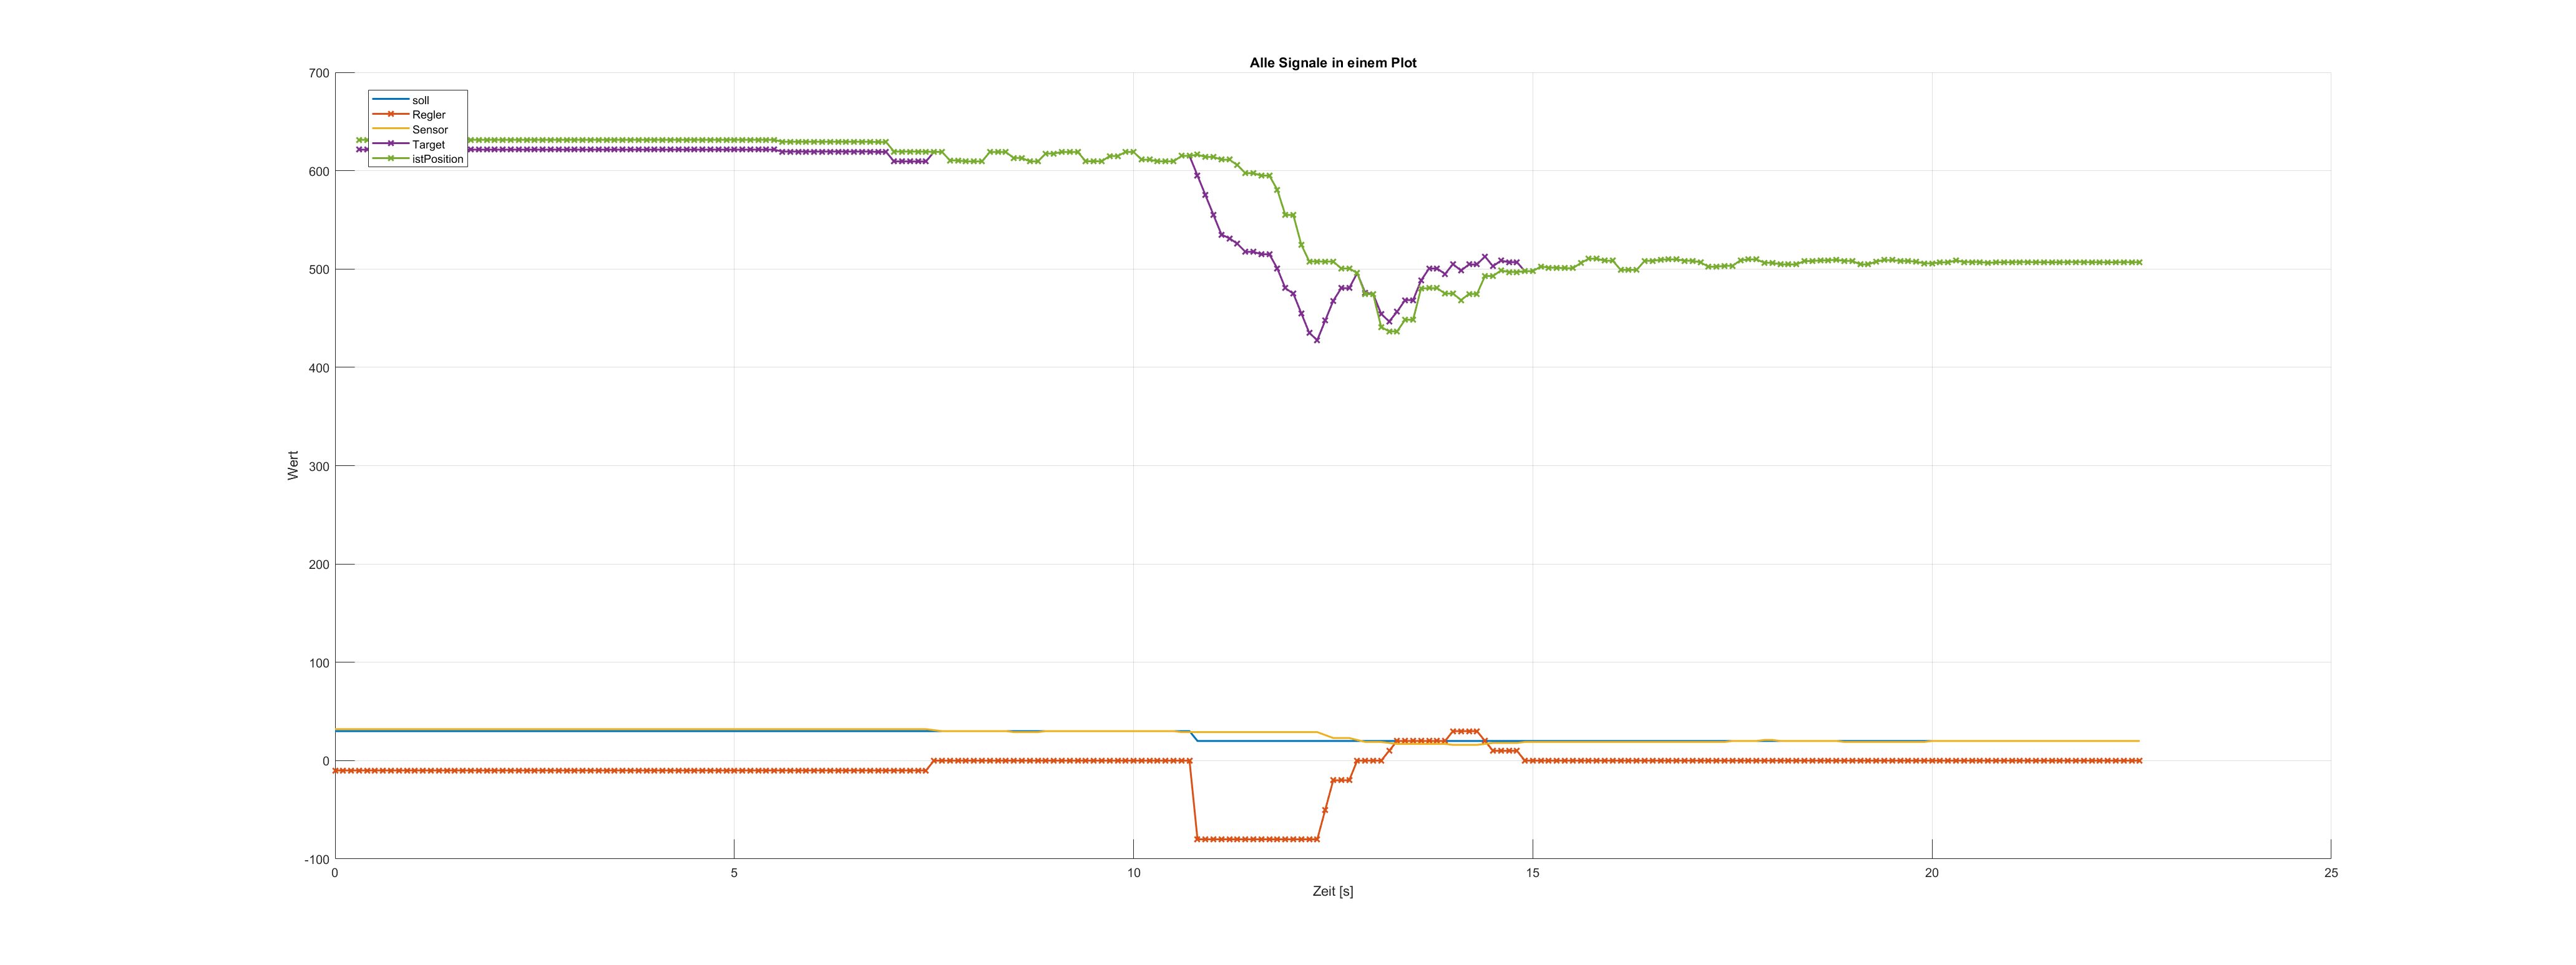
\includegraphics[width=\textwidth]{images/signaleZusammen.png}
        \caption{Siganle übereinander gelegt}
        \label{fig:signaleZusammen} % Label für Teilbild (b)
    \end{subfigure}
    
    \caption{Vergleich von Target- und Ist-Position.}
    \label{fig:signale} % Label für die gesamte Abbildung
\end{figure}

Vergleicht man die Zielposition (\textit{Target}) und die Ist-Position, wird deutlich, dass die Ist-Position dem Target hinterherhinkt [vgl. \ref{fig:signaleZusammen}]. Zudem werden nicht alle Targets angefahren; dies ist daran erkennbar, dass die Target-Werte eine Spitze bei $12{,}8$ aufweisen, die Ist-Positionen diese Spitze jedoch nicht erreichen. Die Grafik legt nahe, dass die Totzeit des Ist-Positionswertes für das starke Überschwingen verantwortlich war.

Wurden zwischen den \texttt{MOVE\_STEP}-Zuständen $30$~Ticks gewartet, fuhr der Arm ohne Überschwingen auf die gewünschte Position. Allerdings benötigte das System diese $30$~Ticks, um eine Signaländerung wahrzunehmen.

